\documentclass[11pt]{article}

\usepackage[left=3cm,right=3cm,top=3cm,bottom=3cm]{geometry}

% For Times New Roman font
\usepackage{mathptmx}

% Packages for formatting
\usepackage{titlesec}
\usepackage{titling}
\usepackage{abstract}

\usepackage{algorithm}
\usepackage{algpseudocode}
\usepackage{float}
\usepackage{anyfontsize}
\usepackage{etoolbox}
\usepackage{graphicx}
\usepackage{tcolorbox}
\usepackage{enumitem}

% Customize section and subsection font sizes
\titleformat{\section}[block]{\normalfont\fontsize{13pt}{15pt}\bfseries}{\thesection}{1em}{}
\titleformat{\subsection}[block]{\normalfont\fontsize{12pt}{14pt}\bfseries}{\thesubsection}{1em}{}

% Change the title font size
\pretitle{\vspace{-6em}\begin{center}\fontsize{14pt}{16pt}\bfseries}
\posttitle{\par\end{center}\vskip 0.5em}

\preauthor{\vspace{0em}\begin{center}\small}
\postauthor{\vspace{-4em}\end{center}}

\renewcommand{\abstractname}{}
\renewcommand{\abstractnamefont}{\normalfont\small\bfseries}
\renewcommand{\abstracttextfont}{\normalfont\small}

% Remove line numbers
\makeatletter
\patchcmd{\algorithmic}{\itemsep\z@}{\itemsep\z@\lineskip\z@}{}{}
\makeatother

\begin{document}

\title{Indexus: A Peer-to-Peer Search Algorithm}
\author{Remi Henriot  \\
        indexus.io }
\date{}

\maketitle

\begin{abstract}
\noindent \textbf{Abstract. }A peer-to-peer protocol engineered to facilitate nearest neighbor and range queries across multi-dimensional datasets. Both node addresses and datasets are mapped onto a unified binary space partitioning (BSP) tree, creating a streamlined and convergent system. The choice of a BSP tree over an R-tree for the data splitting strategy simplifies the protocol by reducing complex node interactions during insertion and deletion operations. The system achieves eventual consistency, high I/O throughput, and robust resilience through the integration of CRDT mechanisms, complemented by strategic caching and replication.
\vspace{1em}\end{abstract}

\section*{Introduction}
In the contemporary digital ecosystem, the concentration of data control by a limited number of centralized entities poses significant risks, including privacy violations and the potential for abuse of power. These entities create systemic vulnerabilities due to their centralized nature, which can lead to significant data breaches and a lack of competitive diversity in the market.

\vspace{1em}

Advancements in decentralized technologies have begun to address these issues by enabling secure, transparent transactions and autonomous data management without centralized oversight. These innovations have facilitated more democratic governance structures and provided mechanisms for asset digitization, contributing to a more equitable digital landscape.

\vspace{1em}

However, a critical challenge persists: the user experience in decentralized systems often lacks the ease and efficiency of data retrieval found in centralized platforms. Centralized systems benefit from advanced indexing systems that facilitate straightforward navigation and information retrieval, a feature decentralized architectures have struggled to match.

\vspace{1em}

To bridge this gap, there is a need for a decentralized protocol that integrates a global indexing layer. Such a protocol would enhance the functionality of decentralized networks, making them more accessible and user-friendly. This improvement is crucial for increasing the adoption of decentralized solutions, thus supporting a shift towards a more distributed and resilient digital infrastructure.

\section*{Objective and Constraints}
We aim to develop a data storage and retrieval system that organizes data in a way that incremental nearby search is possible to mimic existing data feeds. 
If we consider a news feed scroll, it begins at the present moment—the spatial origin—and progresses backward in time. As users scroll, they encounter older news items that are incrementally distanced from the origin.

\vspace{1em}

Any feed, whether it tracks events or operates as part of an online marketplace, can be conceptualized as a single or multi-dimensional incremental search. The underlying data reservoir for these feeds can be vast, necessitating a system that can handle intensive read and write operations robustly. To ensure equitable data access and prevent centralized control, the data should not be localized on a single machine. Instead, it must be distributed across a network of nodes, supporting a decentralized architecture that avoids unfair ownership and enhances system resilience.

\vspace{1em}

For this system, the immediate consistency of the feed is not critical, provided that the data eventually converge to a stable state. This approach allows for eventual consistency across the network, enabling the system to prioritize performance and scalability while ensuring that nodes will ultimately synchronize to reflect coherent information.

\section*{Structure}

The client and node interactions rely on the same data structure: a binary tree representing the encoding space where node addresses, collection IDs, sets, and item locations are materialized by the leaves of the tree. The data structure has been chosen carefully to support collection scalability, search queries, and network routing.

\vspace{1em}

\begin{figure}[H]
    \centering
    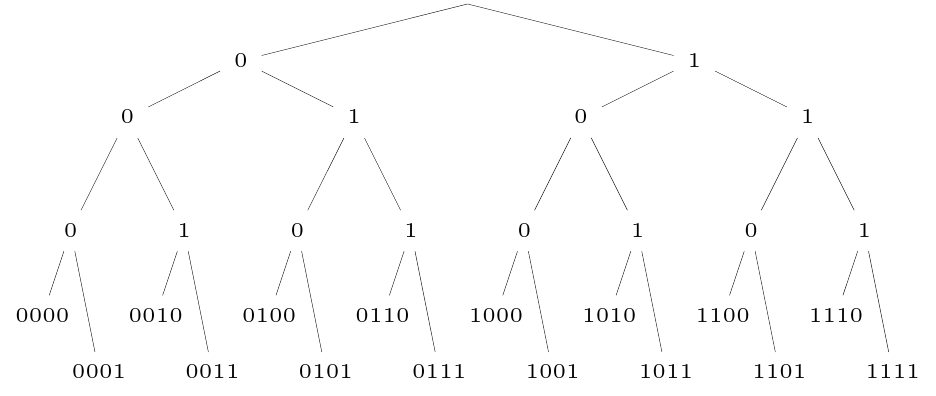
\includegraphics[width=10cm]{tree.png}
    \label{fig:tree}
    \caption{Binary tree}
\end{figure}

\vspace{1em}

Let’s consider a BASE4 system (using symbols A, B, C, and D) for our examples. The size of the base determines the amount of data stored within each set. Typically, we use a base 64 system for greater efficiency.

\vspace{1em}

\begin{figure}[H]
    \centering
    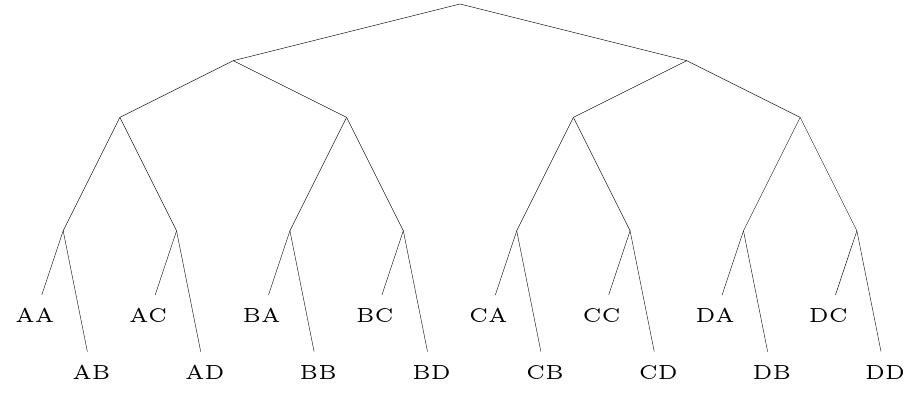
\includegraphics[width=10cm]{encoded.png}
    \label{fig:encoded}
    \caption{Encoded tree (BASE4)}
\end{figure}

\vspace{1em}

\section*{Geometry}
\subsection*{Dimension}
A dimension is defined by a distance function between coordinates. Common examples include time, geographic coordinates, or any other measurable attribute that can be used to organize the data. It usually also embeds filtering and directional functions for range queries.

\subsection*{Space}
A space is a defined multi-dimensional area that encompasses specific ranges for each dimension. It uses a \textbf{mask} and an \textbf{offset} to encode locations within that space.

\vspace{1em}

\noindent The offset is used to randomize the final hash of the location. By introducing randomness, we reduce the likelihood that a single data provider becomes responsible for too much information, especially when multiple collections are involved. This randomization promotes a fair distribution of data across the network nodes.

\vspace{1em}

\noindent The mask maps the coordinates onto the bits of the base encoding. It defines how each bit in the location hash corresponds to the dimensions of the space. The choice of mask is crucial because it affects the number of layers (levels of partitioning) required for the collection. Fewer layers lead to more efficient data retrieval.

\vspace{1em}

\subsection*{Example}

\begin{tcolorbox}[colframe=black!75!black]
\textbf{Geolocation:} Latitude, Longitude\\
\textbf{Base:} ABCD\\
\textbf{Mask:} (0,1,0,1) = (Latitude, Longitude, Latitude, Longitude)\\
\textbf{Offset:} BC
\begin{itemize}[noitemsep, topsep=2pt]
    \item \textbf{1st, 2nd bits:} A: 11, B: 00, C: 01, D: 10
    \item \textbf{3rd, 4th bits:} A: 10, B: 11, C: 00, D: 01
\end{itemize}
\vspace{0.5em}
\textbf{Location:} BD = 0001\\
\textbf{Ranges:}
\begin{itemize}[noitemsep, topsep=2pt]
    \item \textbf{Latitude:} [-90, 90] degrees
    \item \textbf{Longitude:} [-180, 180] degrees
\end{itemize}
\vspace{0.5em}
\textbf{Decoding Steps:}
\begin{itemize}[noitemsep, topsep=2pt]
    \item \textbf{Step 1:} Latitude [-90, 0] (first half)
    \item \textbf{Step 2:} Longitude [-180, 0] (first half)
    \item \textbf{Step 3:} Latitude [-90, -45] (first half)
    \item \textbf{Step 4:} Longitude [-90, 0] (second half)
\end{itemize}
\vspace{0.5em}
\textbf{Result:} BD = Latitude in [-90, -45], Longitude in [-90, 0]
\end{tcolorbox}

\vspace{2em}

\noindent Consider using a BASE64 encoding, which provides 6 bits per layer. This means we can partition our space 6 times consecutively in each layer. By tailoring the bit allocation, we can match the partitioning to the actual data distribution, which can improve both data balance and retrieval efficiency.

\vspace{2em}

\begin{figure}[H]
    \centering
    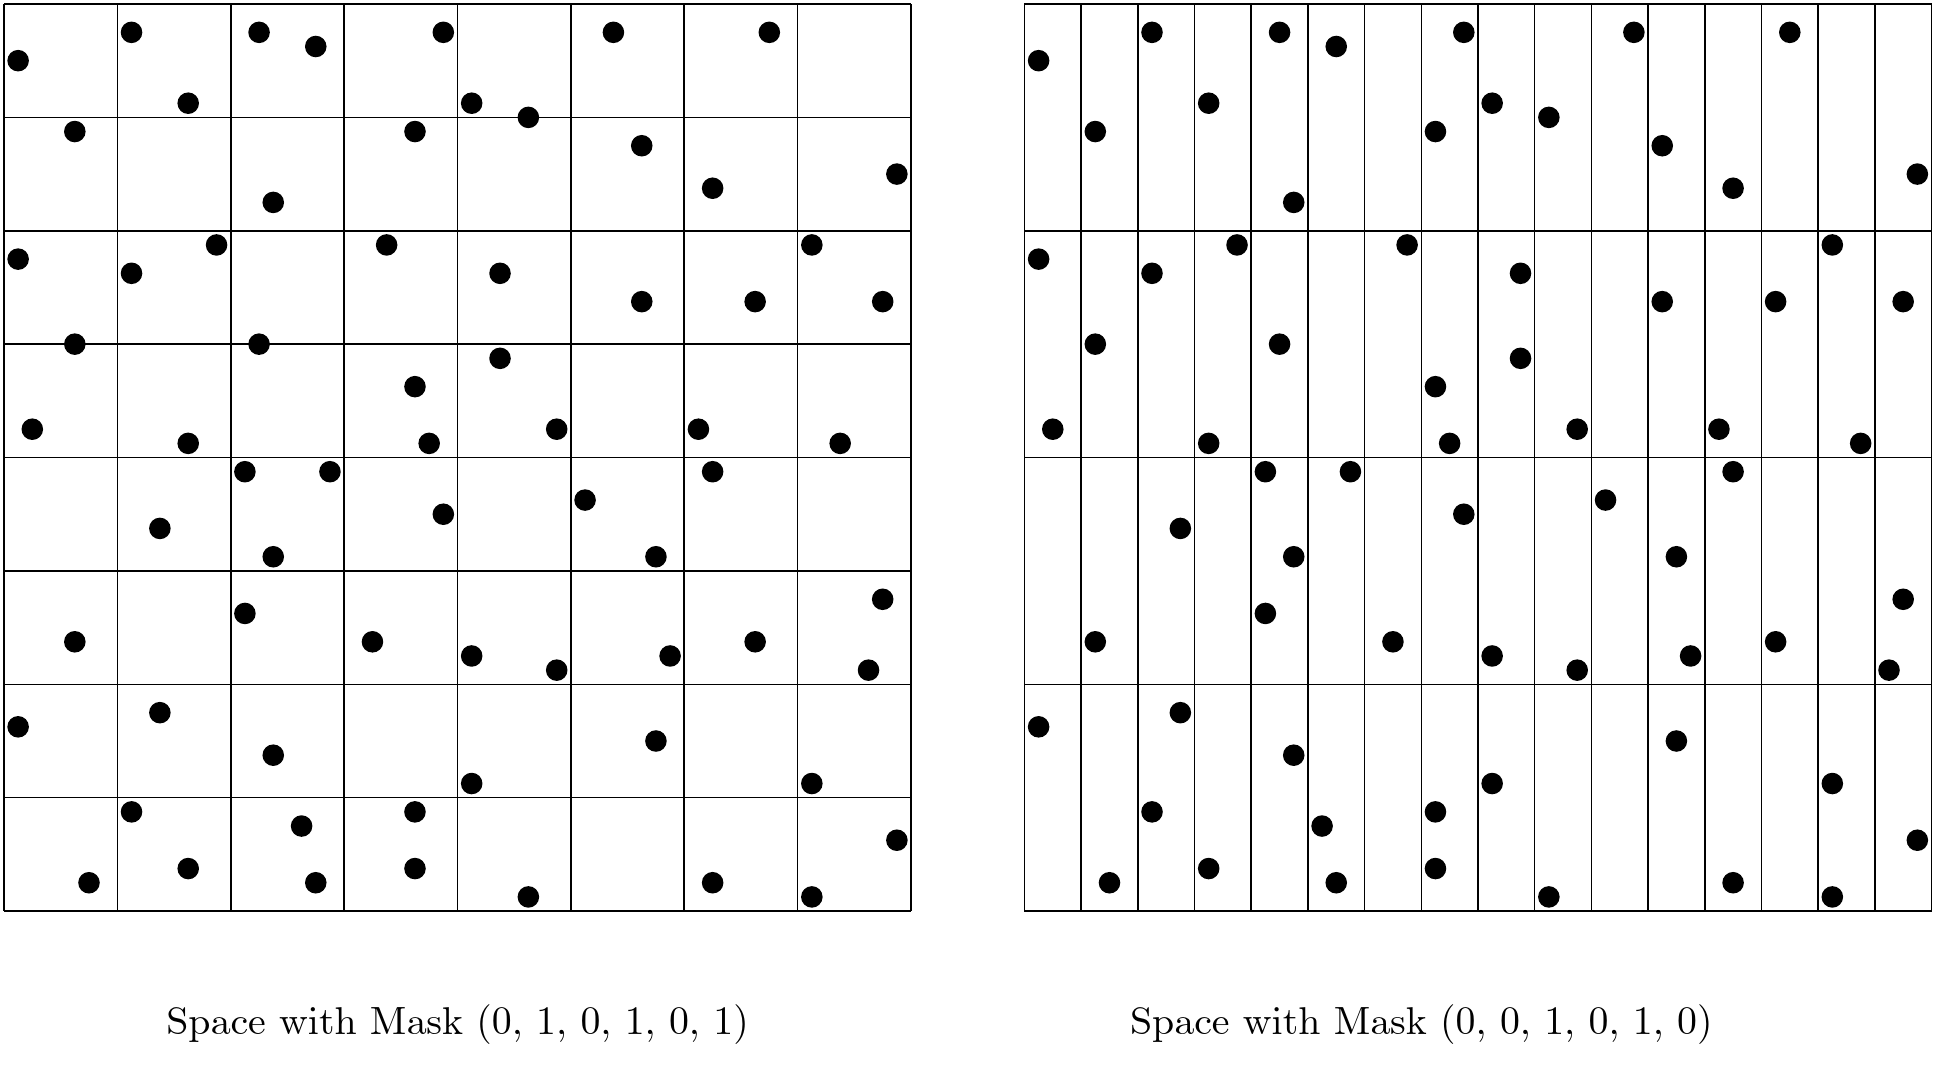
\includegraphics[width=12cm]{masks.png}
    \label{fig:masks}
    \caption{Two subdivisions of the same space}
\end{figure}

\section*{Data}
\subsection*{Item}
An item represents a unit of data within the system. It can be a piece of content, such as a news article, a product listing, or any other discrete piece of information. An item is associated with a unique ID and has coordinates across one or many dimensions.

\subsection*{Collection}
A collection represents a dataset of items within a space. Its definition should contain at least the dimension ranges, metric functions used, the mask to resolve the location, and the delegation threshold. We propose to hash its content and encode it to generate an identifier that will be used as the offset of the space it covers.

\subsection*{Set}
A set represents a partition of a space. It contains a combination of subsets and items defined in the located range. When the number of items and subsets reaches a limit size, subsets are created to group items within child locations, and the parent set is shrunk. This shrinking operation allows the protocol to guarantee a maximum size of the data queried. A parent set and its descendants live within the closest node until the number of child items reaches a predefined threshold that forces the current node to delegate subsets to other nodes. 

\subsection*{Example}
Let's represent a collection and its data with the following parameters - dimensions: 2, base: 4, set size: 10, properties: [count], offset: none.

\vspace{1em}

\begin{figure}[H]
    \centering
    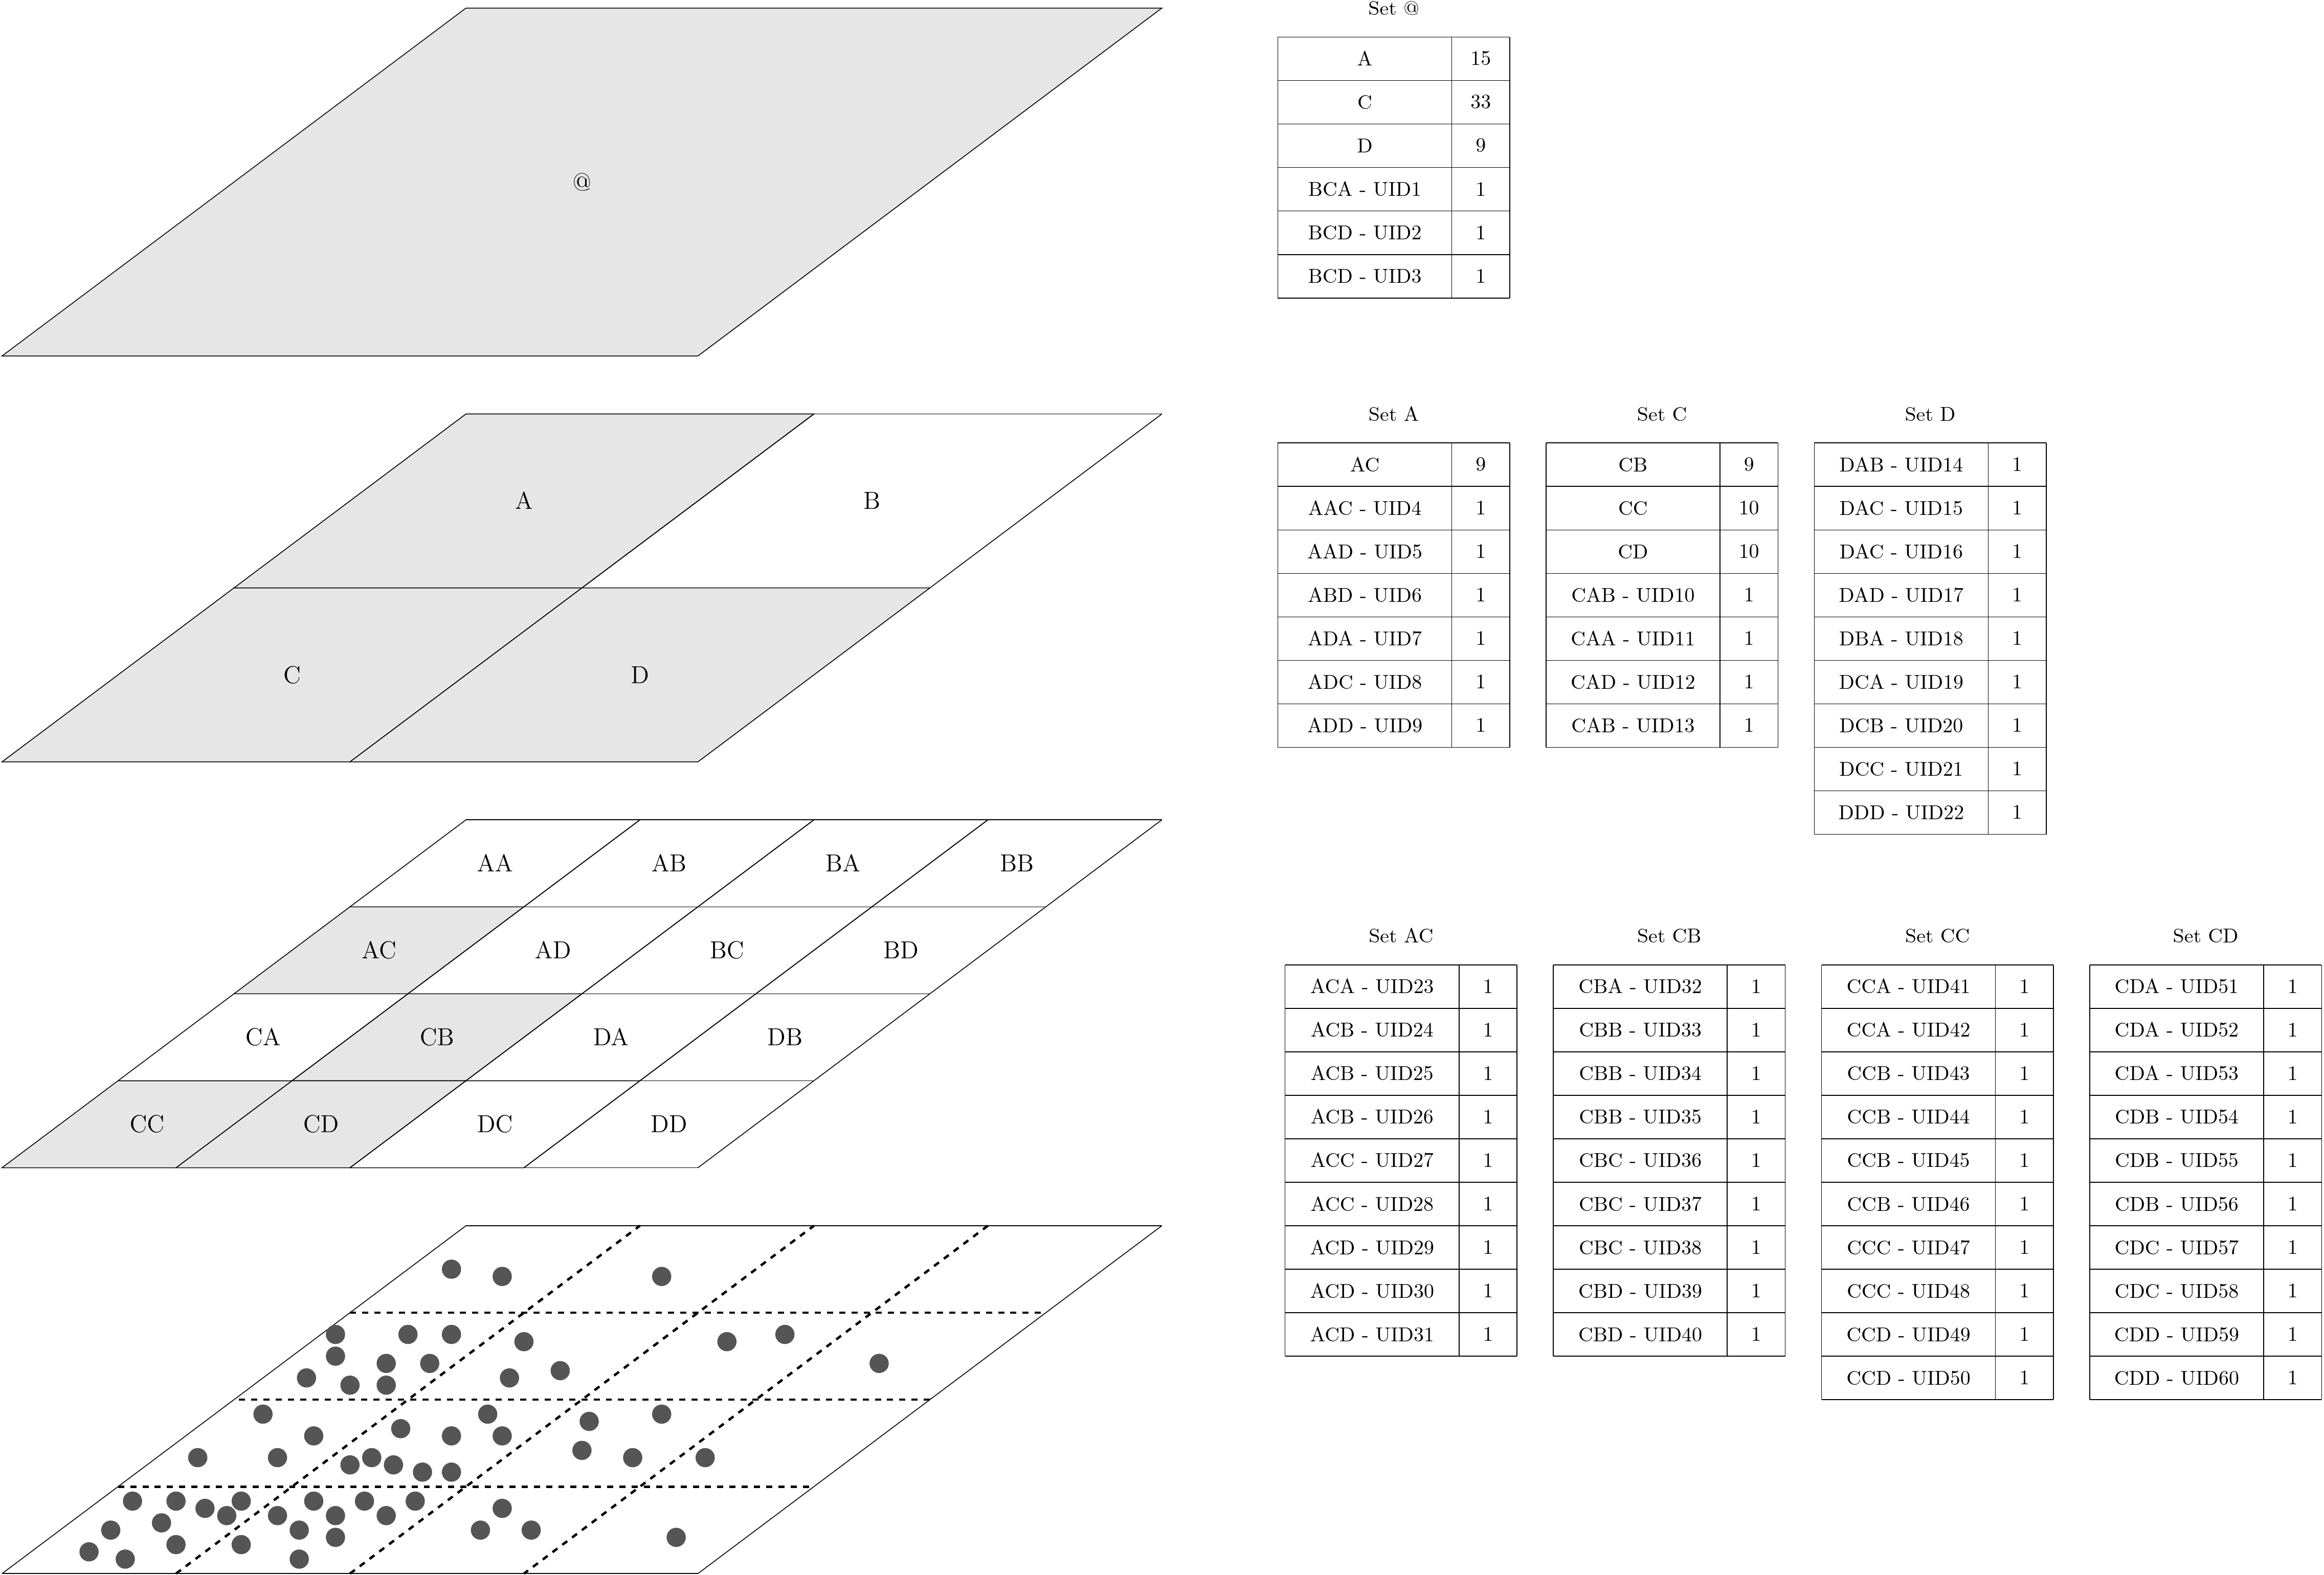
\includegraphics[width=15cm]{collection.png}
    \label{fig:collection}
    \caption{Collection, set, and items}
\end{figure}

\vspace{1em}

\section*{Data Contract}

Let’s consider a system providing data based on the following methods:

\vspace{2em}

\begin{tcolorbox}[colframe=black!75!black]
    \textbf{getSet(collection, location):} Retrieves data from a collection area\\ \\
    \textbf{addItem(collection, location, id):} Adds an identifier into a collection at a specific location.
\end{tcolorbox}

\vspace{1em}

\section*{Search Algorithm}

We want our algorithm to guarantee at least two properties:

\vspace{1em}

\begin{itemize}[noitemsep, topsep=2pt]
    \item \textbf{Incremental item searches within a reasonable time.}
    \item \textbf{Maintain a consistent order of items presented.}
\end{itemize}

\vspace{1em}

\noindent Incremental searches mean loading items in batches of \(N\) items. Ordering implies we can compare items (smaller, greater) and assign each item a distance to an origin. The search performance should be maintained for heterogeneous data distributions.

\subsection*{Metric Space}

Consider geolocated items; the metric space is defined by two coordinates (latitude, longitude), and we can define a function to calculate the distance between two items. The space can also be subdivided into areas as mentioned above.

\vspace{1em}

\noindent We define another method to calculate the distance from a point to an area. If the point is within the area, the distance is 0; if not, we consider the shortest distance to the area.

\subsection*{Search Parameters}

To perform a search, we need to define the following parameters:

\begin{tcolorbox}[colframe=black!75!black]
    \textbf{Origin:} The reference point (e.g., a specific latitude and longitude).\\
    \textbf{Sorting:} The method to sort results (e.g., closest to furthest items).\\
    \textbf{Batch Size:} The number of items to retrieve per batch.\\
    \textbf{Cap:} A tradeoff parameter called Cap to optimize the search.
\end{tcolorbox}

\subsection*{Initialization and Layers}

We initialize our algorithm by adding the root set of the collection into the selected areas to load layer 0. Sets will be stored into different layers based on their precision. We request the data for the root set and receive data back, such as items and subsets, which we then store in child layer 1.

\subsection*{Recursion}

We sort all indexed sets based on their distances to the origin and select sets incrementally until we reach a sum of their counters higher than \texttt{BatchSize} \(\times\) \texttt{Cap}. This threshold mechanism guarantees efficiency by minimizing the rounds of requests—a tradeoff between the number of rounds and the number of requests per round.

If we don't have enough sets (and therefore subsequent items) to reach the threshold, we decrease our layer index to progress and extend our radius on the parent layers. We can recursively apply those steps until the last layer processed generates only items. 

\subsection*{Visualization}

When selecting the sets, we verify the threshold but also ensure that we don't select a set further than the first indexed set of the previous layer. This constraint guarantees we load sets and items gradually and preserve ordering consistency. We can visualize the algorithm as concentric circles, each representing a layer, with its radius being the first set indexed. The circle represents a constraint for child layers. 

\vspace{1em}

\begin{figure}[H]
    \centering
    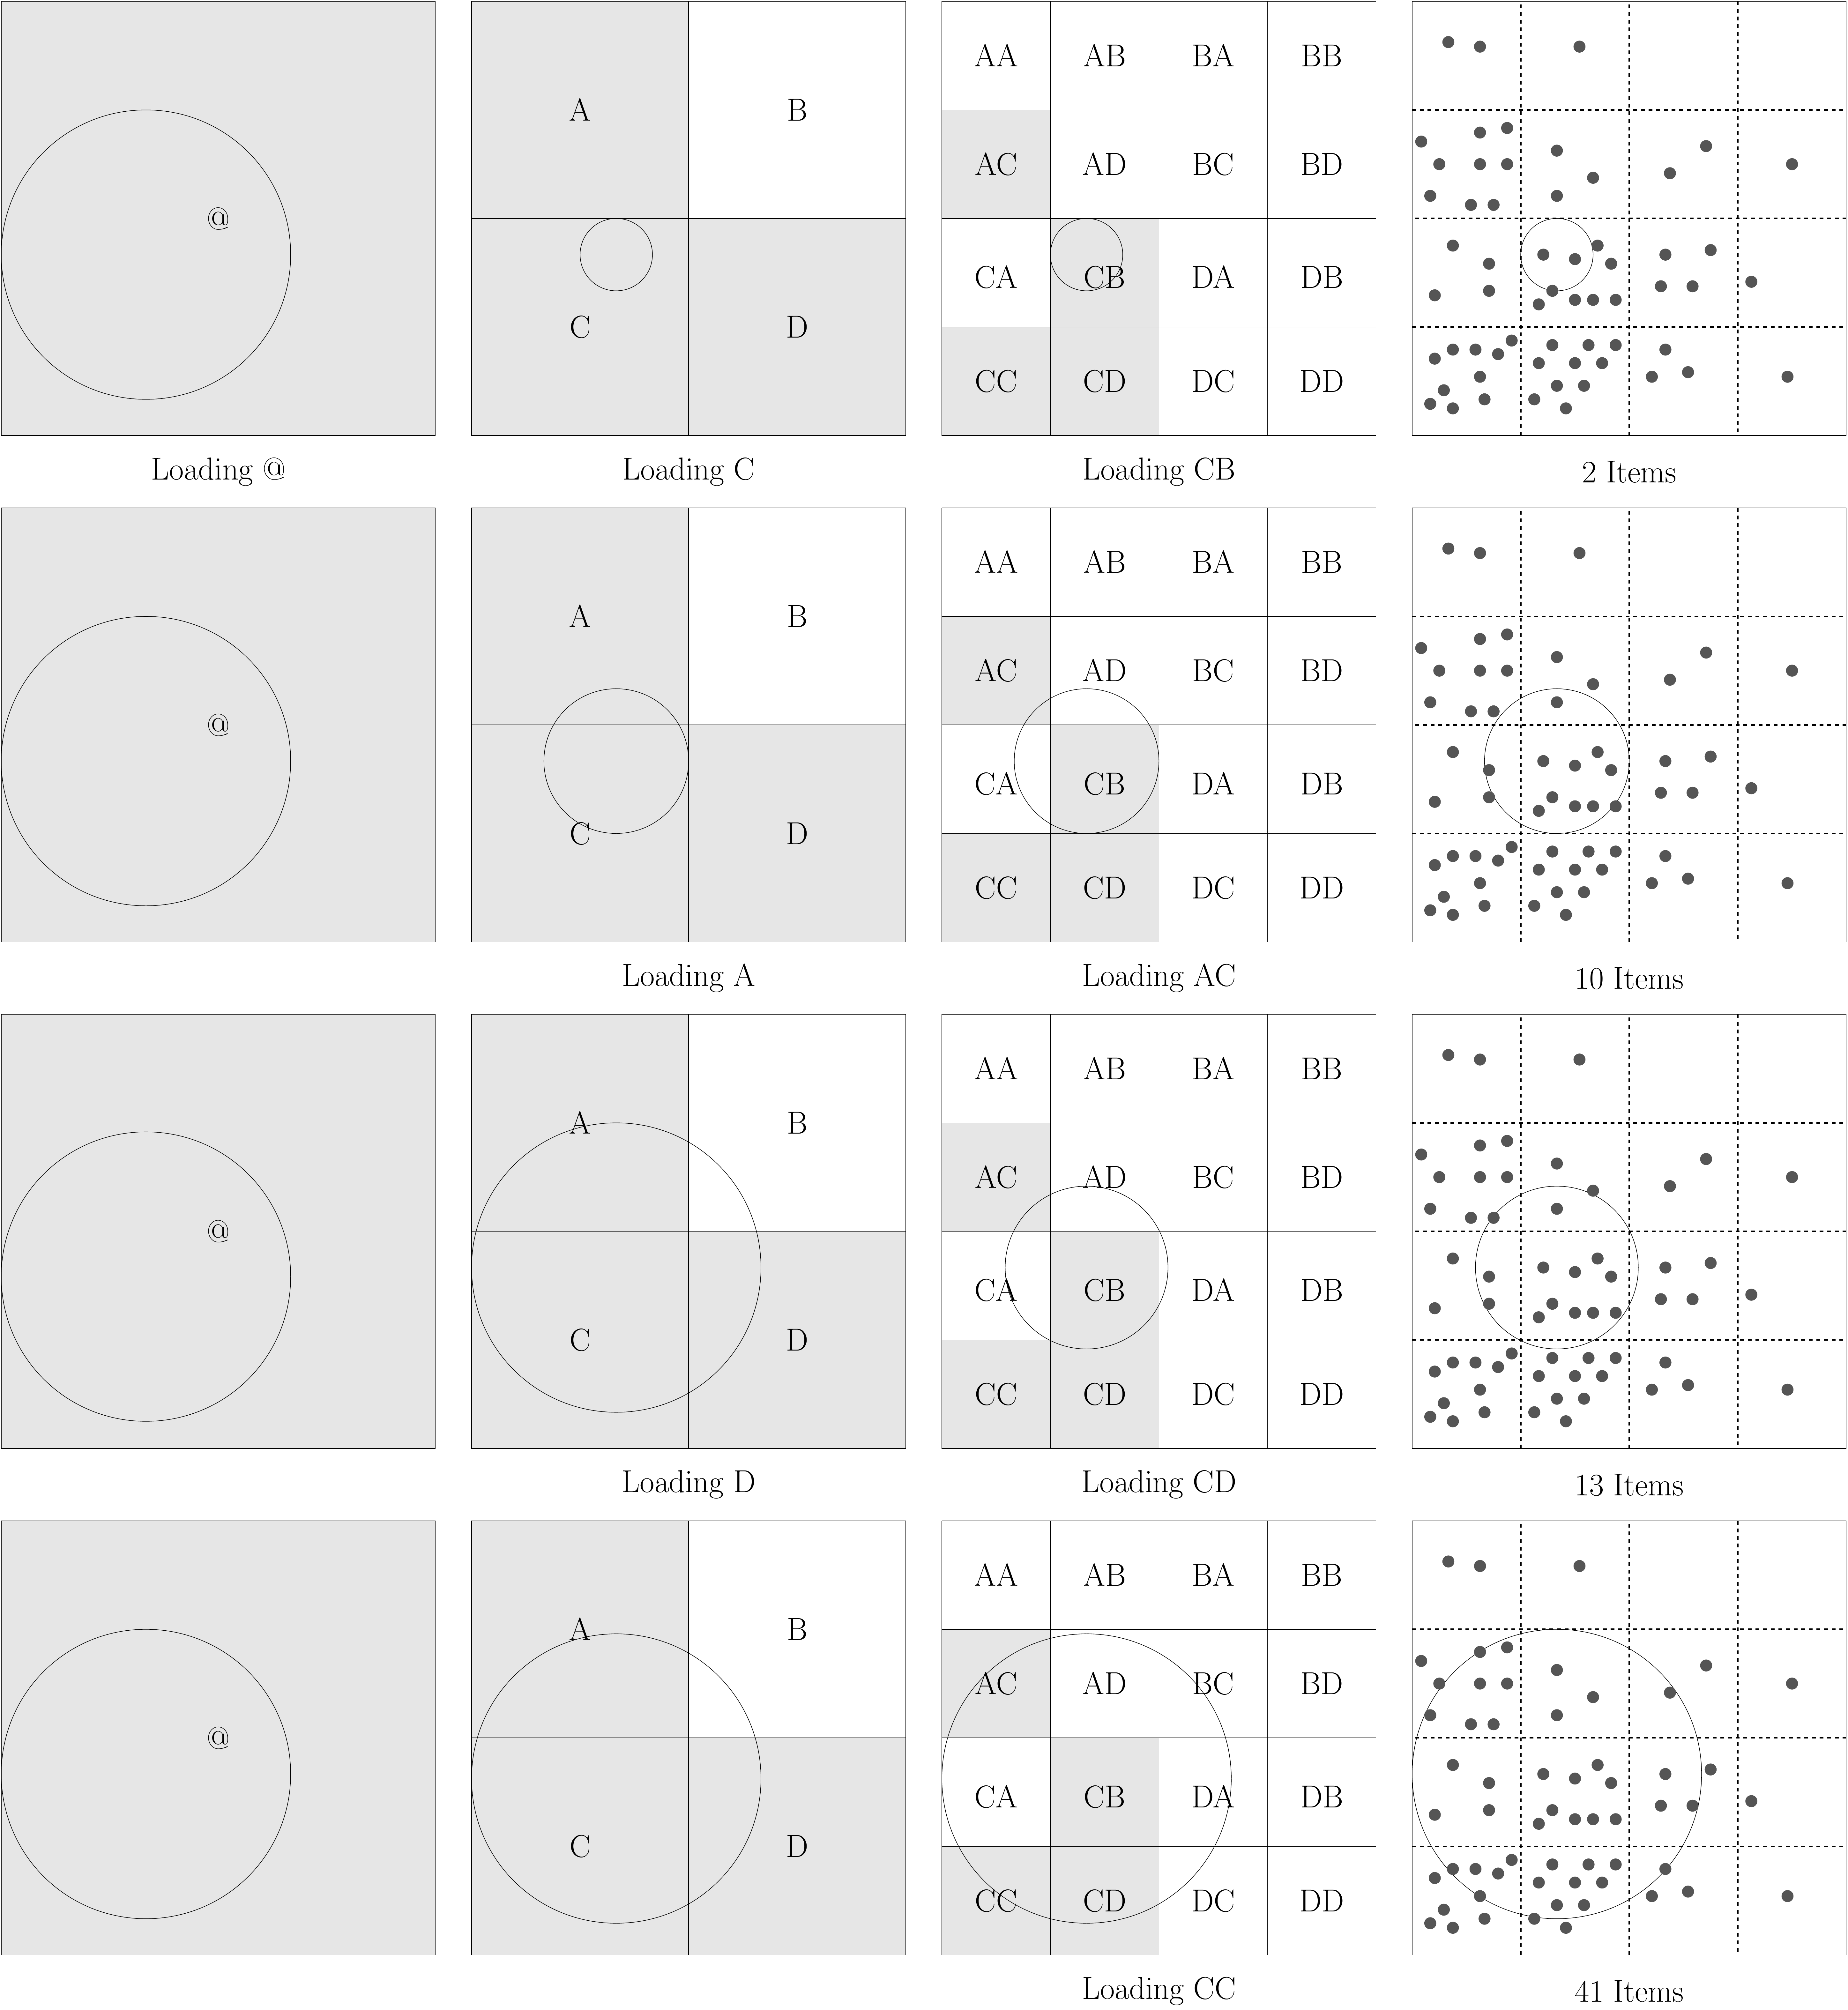
\includegraphics[width=15cm]{layers.png}
    \label{fig:layers}
    \caption{Layers and concentric circles}
\end{figure}

\section*{Detailed Implementation}

\begin{algorithm}[H]
\caption{Search Algorithm}
\label{alg:search}
\begin{algorithmic}[1]
\small
\Function{search}{}
    \If{\Call{prepare}{} is true and c.final is true}
        \State \Call{stream}{}
        \State \Return
    \ElsIf{\Call{prepare}{} is true}
        \State \Call{query}{}
        \State level++
    \Else
        \State level--
        \If{level == 0}
            \State level = \Call{length}{layers}
        \EndIf
    \EndIf
    \State \Call{search}{}
\EndFunction
\State
\Function{prepare}{} $\rightarrow$ Boolean \Comment{c: current, p: previous, n: next layers}
    \State \Call{sort}{c.index}
    \State select, count, items $\leftarrow$ 0, 0, 0
    \For{el in c.index}
        \If{level $>$ 0 and (el.distance $>$ p.radius or count $\geq$ cap $\times$ limit)}
            \State \textbf{break}
        \EndIf
        \If{el is Item}
            \State items++
        \EndIf
        \State \Call{add}{c.select, el}
        \State select++
        \State count += el.Count()
    \EndFor
    \State \Call{remove}{c.index, select, count}
    \If{level == 0}
        \State c.final = false
        \State \Return true
    \EndIf
    \If{c.index.count == 0 or c.index[0].distance $>$ p.radius}
        \State c.radius = p.radius
    \Else
        \State c.radius = c.index[0].distance
    \EndIf
    \State p.waiting = c.index.count + c.waiting
    \State p.load.count = c.index.count + c.select.count + c.load.count
    \State predicted = c.load.count + c.select.count - c.waiting
    \State c.final = c.final and items == select and level + 1 == \Call{length}{layers}
    \State \Return predicted $\geq$ limit or c.radius == first.radius
\EndFunction
\end{algorithmic}
\end{algorithm}

\begin{algorithm}[H]
\caption{Query and Stream Functions}
\begin{algorithmic}[1]
\Function{query}{}
    \For{set in c.select}
        \State result = \Call{getSet}{set}
        \State \Call{add}{n.index, result}
    \EndFor
    \State \Call{concat}{c.load, c.select}
    \State \Call{clear}{c.select}
\EndFunction
\State
\Function{stream}{}
    \For{item in c.select}
        \State output $\gets$ item
    \EndFor
    \State \Call{concat}{c.load, c.select}
    \State \Call{clear}{c.select}
\EndFunction
\end{algorithmic}
\end{algorithm}

\section*{Advanced Topics}

\subsection*{Filtering}

\subsection*{Cross Collections}

\subsection*{Aggregation}
We propose to associate properties with each item; they should be part of an Abelian group so we can compute values for their parent sets. 

\subsection*{Loading}
Based on set properties, faster retrieval and a progressive resolution of the data are possible - blurred to the most detailed one.

\subsection*{Dimensions}

\subsection*{Ratios}
When multi-dimensional sub-distances can be weighted based on user preferences.

\end{document}